%!TEX encoding = UTF-8 Unicode
\documentclass{lecturenotes}

\setbeamertemplate{footline}[frame number]
\title[Scala introduktion]{Introduction to programming using Scala}
\subtitle{-- Experiences from 1st year of new course for CSE students}
\author{Björn Regnell}
\institute{Dept. of Computer Science, LTH \\ Lund University, Sweden \\ \vspace{1em}Download slides:\\ \url{https://github.com/lunduniversity/introprog/blob/master/about/course-experience-first-year}}
\date{\today}

\newcommand{\Section}[1]{\section{#1}\frame{\centering\huge\bfseries\textcolor{blue}{#1}}}

\usepackage{tikz}
\usepackage{pgfplots}
%&\pgfplotsset{compat=newest}
\pgfplotsset{compat=1.14}
\usepackage{pgfplotstable}

\usepackage{filecontents}

%http://tex.stackexchange.com/questions/135393/how-to-draw-bar-pie-chart
\definecolor{c1}{RGB}{220,57,18}
\definecolor{c2}{RGB}{255,153,0}
\definecolor{c3}{RGB}{102,140,217}
\definecolor{c4}{RGB}{16,150,24}
\definecolor{c5}{RGB}{153,0,153}




\makeatletter

\tikzstyle{chart}=[
    legend label/.style={font={\scriptsize},anchor=west,align=left},
    legend box/.style={rectangle, draw, minimum size=5pt},
    axis/.style={black,semithick,->},
    axis label/.style={anchor=east,font={\tiny}},
]

\tikzstyle{bar chart}=[
    chart,
    bar width/.code={
        \pgfmathparse{##1/2}
        \global\let\bar@w\pgfmathresult
    },
    bar/.style={very thick, draw=white},
    bar label/.style={font={\bf\small},anchor=north},
    bar value/.style={font={\footnotesize}},
    bar width=.75,
]

\tikzstyle{pie chart}=[
    chart,
    slice/.style={line cap=round, line join=round, very thick,draw=white},
    pie title/.style={font={\bf}},
    slice type/.style 2 args={
        ##1/.style={fill=##2},
        values of ##1/.style={}
    }
]

\pgfdeclarelayer{background}
\pgfdeclarelayer{foreground}
\pgfsetlayers{background,main,foreground}


\newcommand{\pie}[3][]{
    \begin{scope}[#1]
    \pgfmathsetmacro{\curA}{90}
    \pgfmathsetmacro{\r}{1}
    \def\c{(0,0)}
    \node[pie title] at (90:1.3) {#2};
    \foreach \v/\s in{#3}{
        \pgfmathsetmacro{\deltaA}{\v/100*360}
        \pgfmathsetmacro{\nextA}{\curA + \deltaA}
        \pgfmathsetmacro{\midA}{(\curA+\nextA)/2}

        \path[slice,\s] \c
            -- +(\curA:\r)
            arc (\curA:\nextA:\r)
            -- cycle;
        \pgfmathsetmacro{\d}{max((\deltaA * -(.5/50) + 1) , .5)}

        \begin{pgfonlayer}{foreground}
        \path \c -- node[pos=\d,pie values,values of \s]{$\v\%$} +(\midA:\r);
        \end{pgfonlayer}

        \global\let\curA\nextA
    }
    \end{scope}
}

\newcommand{\legend}[2][]{
    \begin{scope}[#1]
    \path
        \foreach \n/\s in {#2}
            {
                  ++(0,-10pt) node[\s,legend box] {} +(5pt,0) node[legend label] {\n}
            }
    ;
    \end{scope}
}



\begin{document}

\frame{\titlepage}
\frame{\tableofcontents}

%%% EXPERIENCES

\Section{Why a new course?}

\begin{Slide}{Why a new programming course for CSE students?}

\begin{itemize}
\item Special teaching challenges when teaching introductory programming to CSE\footnote{CSE = Computer Sci. \& Eng., In Swedish: Datateknikprogrammet (D)} program students at LTH:
\begin{itemize}
\item Very large spread in pre-knowledge
\item Many students have very high ambitions
\item Some students have great difficulties
\end{itemize}
\item The previous first course EDA016 needed an update after having the same architecture for many years
\end{itemize}
\end{Slide}

\begin{Slide}{Course intro survey 2015, CSE (Datateknik)\\EDA016 Programming, first course (Java)}
\begin{multicols}{2}
Have programmed before? \vspace{1em}

\includegraphics[width=0.55\textwidth]{img/survey-2015}
\columnbreak

\raggedleft What language?  \vspace{1em}

\includegraphics[width=0.55\textwidth]{img/lang-2015}
\end{multicols}
\end{Slide}


\begin{Slide}{Course results 2015, CSE (Datateknik)\\EDA016 Programming, first course (Java)}
%\begin{multicols}{2}

Grades 2015, old Java course,  91 students attending first exam
\vspace{2em}

\includegraphics[width=0.55\textwidth]{img/grades-2015}

%\columnbreak

%\raggedleft \Emph{Goal of 2016} \\
%To \Alert{increase} the \\ \Alert{challenge level} \& \\  \Alert{learning outcome} \\ significantly.
%\end{multicols}
\end{Slide}

\begin{Slide}{Main goals with new course}\small
\begin{itemize}
\item Increase the \Emph{challenge}
\item Increase the \Emph{learning outcome}
\item Make an \Emph{interesting \& engaging} start for CSE students
\item Try new concepts in introductory programming teaching:
\begin{itemize}
\item Involve old students in an open source project
\item Increase learning collaboration among students
\item Pioneering Scala as a first language
\end{itemize}
\item Enable students to continue with an unchanged second course
\end{itemize}
\end{Slide}


\begin{Slide}{First language at LTH}%\small
History of first languages at LTH for CSE students:
\begin{table}
\begin{tabular}{l l}
(Algol, Fortran) & (pre-history\footnote{Prof. Martin Odersky at EPFL, the inventor of Scala, wrote large parts of the javac compiler. He was once a PhD student of Niklaus Wirth, the chief designer behind Algol, Pascal, Modula etc.} using punch cards) \\
 Pascal & 1982, CSE program started\\
 Simula &  1990 \\
Java &  1997 \\
\textbf{Scala} &  2016 \\
\end{tabular}
\end{table}

\end{Slide}



\Section{Why Scala?}

\begin{Slide}{Why Scala?}
Easy for beginners and interesting for non-beginners:
\begin{itemize}
\item Regular semantics; e.g. value types are real objects
\item Concise, expressive syntax
\item Interactive learning in the Scala REPL
\item Multi-paradigm, pragmatic: \\ imperative, object-oriented, functional
\item Rich semantics: can demonstrate many cs concepts
\item Modern, evolving language: exciting for new students
\item Free, open source language and tools
\end{itemize}
%Potential \Alert{risks}:
%\begin{itemize}\fontsize{9}{10}\selectfont
%\item Tools not becoming mature fast enough?
%\item Lack of beginner-oriented teaching material?
%\item Future industrial relevance?
%\item Critical mass of community?
%\end{itemize}
\end{Slide}


%%
\begin{Slide}{What is Scala?}
\begin{itemize}
\item A scalable, pragmatic, real-world language
\begin{itemize}
\item Used at Twitter, LinkedIn, The Guardian, Coursera...
\end{itemize}

\item Multi-paradigm:
\begin{itemize}
\item object-oriented
\item functional
\item imperative
\item concurrent
\end{itemize}
\item Typing: static, strong, inferred, structural

\item Designed by: Martin Odersky
\item Developer: EPFL, Lightbend, OSS Community
\item First appeared:  January 20, 2004
\item Platform: JVM, JavaScript
\item License: BSD 3-clause
\item Official site: \url{https://www.scala-lang.org/}
\end{itemize}
\end{Slide}


\Section{Overview of new course}

\begin{Slide}{Summary of major changes}\footnotesize
\begin{itemize}
\item New contents (selected):
\begin{itemize}\footnotesize
\item Start imperative and functional, then gradually introduce OO
\item Start with objects as modules before instances
\item Immutable versus immutable datastructures
\item Use (but not implement) several structures: Vector, Set, Map, List
\item Use higher-order collection methods: map, foreach, filter, ...
\item Pattern matching to decompose data in case classes
\item Concept focus: compare paradigms, compare languages
\item ...
\end{itemize}
\item Scala as a \Emph{first} language, with Java as a \Alert{second} language in the same course to make concept learning deeper
\item Learning to code in collaboration teams
\item New open source course material:
\begin{itemize}\footnotesize
\item New lectures
\item New exercises
\item New labs
\item New type of written exam
\end{itemize}
\end{itemize}
\end{Slide}

\begin{Slide}{Module structure (adapted based on experiences)}
Home: \textbf{\url{https://lunduniversity.github.io/pgk}} \\ \vspace{1em}

\noindent\resizebox{0.8\columnwidth}{!}{\fontsize{8}{10}\selectfont
%!TEX encoding = UTF-8 Unicode
\begin{tabular}{l|l|l|l}
\textit{W} & \textit{Modul} & \textit{Övn} & \textit{Lab} \\ \hline \hline
W01 & Introduktion & expressions & kojo \\
W02 & Program och kontrollstrukturer & programs & -- \\
W03 & Funktioner och abstraktion & functions & irritext \\
W04 & Objekt och inkapsling & objects & blockmole \\
W05 & Klasser och datamodellering & classes & blockbattle0 \\
W06 & Mönster och felhantering & patterns & blockbattle1 \\
W07 & Sekvenser och enumerationer & sequences & shuffle \\
TP & -- & -- & -- \\
W08 & Nästlade och generiska strukturer & matrices & life \\
W09 & Mängder och tabeller & lookup & words \\
W10 & Arv och komposition & inheritance & snake0 \\
W11 & Varians och kontextparametrar & context & snake1 \\
W12 & Fördjupning, Projekt & extra & Projekt0 \\
W13 & Repetition & examprep & Projekt1 \\
W14 & MUNTLIGT PROV & Munta & Munta \\
TP & VALFRI TENTAMEN & -- & -- \\
\end{tabular}

}
\end{Slide}

\begin{Slide}{Students participation in teaching development through open sourcing of teaching material for Scala}

\textbf{\url{https://github.com/lunduniversity/introprog}}

\begin{multicols}{3}\footnotesize
Anders Buhl, \\Anna Palmqvist Sjövall, \\Anton Andersson, \\Casper Schreiter, \\Cecilia Lindskog, \\Christine Boghammar, \\Emil Wihlander, \\Emma Asklund, \\Erik Bjäreholt, \\Erik Grampp, \\Erik Söderberg, \\Filip Stjernström, \\Fredrik Danebjer, \\Gustav Cedersjö, \\Henrik Olsson, \\Jacob Bohlin, \\Jakob Hök, \\Johan Ravnborg, \\Jonas Danebjer, \\Maj Stenmark, \\Maximilian Rundgren, \\Måns Magnusson, \\Oscar Sigurdsson, \\Oskar Berg, \\Oskar Widmark, \\Povel Larsson, \\Sebastian Hegardt, \\Stefan Jonsson, \\Tom Postema, \\Valthor Halldorsson, \\Viktor Claesson
\end{multicols}

\end{Slide}



\Section{Experiences from first year}


\begin{Slide}{Summary of experiences}
\begin{itemize}
\item Goals met:
\begin{itemize}
\item Students with different pre-knowledge were all challenged
\item Higher learning outcome
\item Increased student engagement
\end{itemize}
\item Scala is an excellent first language for CSE students\\ and a pleasant to teach
\end{itemize}
\end{Slide}

\begin{Slide}{Course Experience Questionnaire}
\begin{multicols}{2}

CEQ 2015 Old Java course
\begin{figure}
\includegraphics[width=0.4\textwidth]{img/CEQ-2015}
\end{figure}
\columnbreak

CEQ 2016 New Scala course

\begin{figure}
\includegraphics[width=0.4\textwidth]{img/CEQ-2016}
\end{figure}

\end{multicols}
\end{Slide}


\begin{Slide}{Betygsfördelning, D-are, totalt 86 st}

%\vspace*{1cm}

2015, 91st

\pgfplotstableread{
betyg antal
0 12
3 04
4 26
5 49
}{\mydataFifteen}

\begin{minipage}{0.4\textwidth}
\hspace*{-0.0cm}
\begin{tikzpicture}[scale=0.8, every node/.style={scale=0.8}]
    \begin{axis}[
            ybar,
            bar width=.5cm,
            width=\textwidth,
            height=0.9\textwidth,
            symbolic x coords={0,3,4,5},
            xtick=data,
            nodes near coords,
            nodes near coords align={vertical},
            ymin=0,ymax=50,
            ylabel={Antal},
            xlabel={Betyg},
        ]
        \addplot table[x=betyg,y=antal]{\mydataFifteen};
    \end{axis}
\end{tikzpicture}
\end{minipage}%
\begin{minipage}{0.3\textwidth}
\vspace*{-1cm}\hspace*{0.5cm}
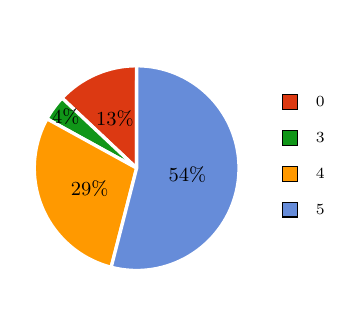
\begin{tikzpicture}
[
    pie chart,
    slice type={NOLL}{c1},
    slice type={TRE}{c4},
    slice type={FYRA}{c2},
    slice type={FEM}{c3},
    pie values/.style={font={\small}},
    scale=1.3, every node/.style={scale=0.8}
]
    \pie{}{13/NOLL,4/TRE,29/FYRA,54/FEM}
    \legend[shift={(1.5cm,1cm)}]{{0}/NOLL,{3}/TRE, {4}/FYRA, {5}/FEM}
\end{tikzpicture}
\end{minipage}%

\vspace*{1em}

2016, 86st
\pgfplotstableread{
betyg antal
0 17
3 12
4 29
5 28
}{\mydataSixteen}

\begin{minipage}{0.4\textwidth}
\hspace*{-0.0cm}
\begin{tikzpicture}[scale=0.8, every node/.style={scale=0.8}]
    \begin{axis}[
            ybar,
            bar width=.5cm,
            width=\textwidth,
            height=0.9\textwidth,
            symbolic x coords={0,3,4,5},
            xtick=data,
            nodes near coords,
            nodes near coords align={vertical},
            ymin=0,ymax=50,
            ylabel={Antal},
            xlabel={Betyg},
        ]
        \addplot table[x=betyg,y=antal]{\mydataSixteen};
    \end{axis}
\end{tikzpicture}
\end{minipage}%
\begin{minipage}{0.3\textwidth}
\vspace*{-1cm}\hspace*{0.5cm}
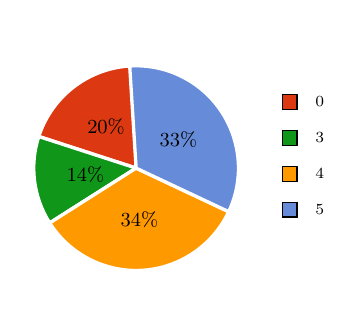
\begin{tikzpicture}
[
    pie chart,
    slice type={NOLL}{c1},
    slice type={TRE}{c4},
    slice type={FYRA}{c2},
    slice type={FEM}{c3},
    pie values/.style={font={\small}},
    scale=1.3, every node/.style={scale=0.8}
]
    \pie{}{20/NOLL,14/TRE,34/FYRA,33/FEM}
    \legend[shift={(1.5cm,1cm)}]{{0}/NOLL,{3}/TRE, {4}/FYRA, {5}/FEM}
\end{tikzpicture}
\end{minipage}%


\end{Slide}



\begin{Slide}{Grade progress 2015:\\EDA016 Java => EDAA01 Java}
\includegraphics[width=1.05\textwidth]{img/2015}
\end{Slide}

\begin{Slide}{Grade progress 2016:\\EDAA45 Scala => EDAA01 Java}
\includegraphics[width=1.05\textwidth]{img/2016}
\end{Slide}



\begin{Slide}{''I learn fast if I make an effort''}
\begin{center}
\includegraphics[width=\textwidth]{img/Q-learn-quick}
\end{center}
\end{Slide}


\begin{Slide}{''I learn fast if I make an effort''}
\begin{center}
\includegraphics[width=\textwidth]{img/Q-learn-quick}
\end{center}
\end{Slide}

\begin{Slide}{''How did you make it at the diagnostic mid-term test?''}
\begin{center}
\includegraphics[width=\textwidth]{img/Q-kontroll}
\end{center}
\end{Slide}

\begin{Slide}{''What did you think about the level of the exam?''}
\begin{center}
\includegraphics[width=\textwidth]{img/Q-exam-hard}
\end{center}
\end{Slide}

\begin{Slide}{''Scala or Java?''}
\begin{center}
\includegraphics[width=\textwidth]{img/Q-scala}
\end{center}
\end{Slide}

\begin{Slide}{''What do you think about the course tempo?''}
\begin{center}
\includegraphics[width=\textwidth]{img/Q-tempo}
\end{center}
\end{Slide}


\begin{Slide}{''How do you value your learning outcome?''}
\begin{center}
\includegraphics[width=\textwidth]{img/Q-learned}
\end{center}
\end{Slide}

\Section{A very brief intro to Scala}

\begin{Slide}{Official home of Scala}
\begin{multicols}{2}
\includegraphics[width=0.5\textwidth]{../../img/scala-logo}

\columnbreak

\hfill\vfill{\large\url{www.scala-lang.org}}\\ with tutorials, docs, etc.

\end{multicols}
\end{Slide}

%%
\begin{Slide}{Scala -- the simple parts}
\fontsize{9}{11}\selectfont
Lecture by \Emph{Martin Odersky}: \href{https://www.youtube.com/watch?v=ecekSCX3B4Q}{www.youtube.com/watch?v=ecekSCX3B4Q}

\begin{multicols}{2}
\fontsize{9}{11}\selectfont
Scala for every-day dev actions:

\begin{enumerate}
\item \Emph{Compose:} everything is a composable \Alert{expression}
\item \Emph{Match:} decompose data with \Alert{pattern}-matching
\item \Emph{Group:} everything can be grouped and \Alert{nested}
\item \Emph{Recurse:} compose at any depth, loop with tail recursion
\item \Emph{Abstract:} functions are objects
\item \Emph{Aggregate:} collections aggregate \& \Alert{transform} data
\item \Emph{Mutate:} local, private mutability to optimize perf.
\end{enumerate}

\columnbreak

\includegraphics[width=0.62\textwidth]{img/odersky}

\end{multicols}
\end{Slide}

\begin{Slide}{Some similarities between Scala and Java}
\begin{itemize}
\item Both are object-oriented and imperative
\item Both are statically typed (\code{~} 100 times faster than Python)
\item Both have C-like block syntax \code+{ }+
\item Both have lambdas (Java 8)
\item Both run on the JVM
\item Both can execute each other's byte code
\end{itemize}
\end{Slide}


\begin{Slide}{Some differences between Scala and Java}\footnotesize
\begin{itemize}
\item Scala is a more ''pure'' OO language: \\ instances of \Emph{\code{Int, Double, Char}}, etc. are \Alert{real objects}
\item Scala is a more advanced functional language: \\ easy to transform immutable data in functional collections
\item Scala unifies OO and functional programming: \\ functions are objects with an \code{apply}-method
\item singelton \code{object} instead of Java's \code{static}

\item Some syntax differences: \pause
\begin{itemize}\fontsize{8}{9}\selectfont
\item semicolons are inferred; newline btw statements is enough
\item no need for \code{return} as blocks are values
\item Type \emph{after} names and colon: \code{val name: String = "Kim"}
\item generic types in \code{[T]} instead of \code{<T>}
\item Five types of members: \code{def, val, lazy val, var, type}
\\ Methods: \code{def isChild: Boolean = age < 18}
\\ Immutable fields: \code{val gender = "Female"}
\\  Delayed init: \code{lazy val r = List.fill(1000)(math.random())}
\\  Mutable fields: \code{var age: Int = 42}
\\  Type alias: \code{type Matrix = Map[Int, Map[Int, String]]}
\end{itemize}


\end{itemize}

\end{Slide}

\begin{Slide}{Classes in Java and Scala}
\vspace{-1.5em}
\begin{multicols}{2}

\javainputlisting{code/JPerson.java}

\columnbreak

\pause

\scalainputlisting{code/SPerson.scala}

\pause

\scalainputlisting{code/Person.scala}

\end{multicols}

\end{Slide}


\begin{Slide}{Live coding: code-along}
Start the REPL:
\begin{REPL}
$ scala
Welcome to Scala 2.11.8 (Java HotSpot(TM) VM, Java 1.8.0_66).
Type in expressions for evaluation. Or try :help.

scala> case class Person(name: String, age: Int = 42)
defined class Person

scala> Person("Björn", 48)
res0: Person = Person(Björn,48)

scala> Person("Kim")
res1: Person = Person(Kim,42)
\end{REPL}

\end{Slide}


\begin{Slide}{Functions are first-class values; Try this in REPL:}
\begin{REPL}[basicstyle=\color{white}\ttfamily\fontsize{8.5}{10}\selectfont]
def öka(i: Int) = i + 1

val nums = Vector(1, 2, 3, 4, 42)

nums.map(öka)

nums.map(i => i + 1)

nums.map(_ + 1)

def mappa(xs: Vector[Int], f: Int => Int) = xs.map(f)

mappa(nums, öka)

def upprepa(n: Int)(block: => Unit) = for (i <- 1 to n) block
\end{REPL}

\end{Slide}




\begin{Slide}{Recommended book for further reading}

\begin{center}
''Programmin in Scala'', 3rd Ed., by Odersky et al.\\
{\small\url{https://www.artima.com/shop/programming\_in\_scala\_3ed}}
\begin{figure}
\includegraphics[width=3cm]{img/pinsbook}
\end{figure}
First edition available online:\\ {\small\url{http://www.artima.com/pins1ed/}}
\end{center}
\end{Slide}

\section*{Q\&A}
\begin{Slide}{Questions?}
\begin{center}
\url{bjorn.regnell@cs.lth.se}
\end{center}
\end{Slide}


\end{document}
